\documentclass{article}

\usepackage{arxiv}
\usepackage[utf8]{inputenc} % allow utf-8 input
\usepackage[T1]{fontenc}    % use 8-bit T1 fonts
\usepackage{hyperref}       % hyperlinks
\usepackage{url}            % simple URL typesetting
\usepackage{booktabs}       % professional-quality tables
\usepackage{amsfonts}       % blackboard math symbols
\usepackage{nicefrac}       % compact symbols for 1/2, etc.
\usepackage{microtype}      % microtypography
\usepackage{lipsum}
\usepackage{graphicx}

\usepackage{gensymb}
\usepackage{lineno}
\usepackage{setspace}

\title{Deep learning and Trajectory Representation for the Prediction of Seabird Diving Behaviour}

\author{
  Amédée Roy \\
  Institut de Recherche pour le Développement,\\
  UMR248 MARBEC (IRD/CNRS/IFREMER/UM)\\
  Avenue Jean Monnet, 34200, Sète, France \\
  \texttt{amedee.roy@ird.fr} \\
   \And
  Sophie Bertrand \\
  Institut de Recherche pour le Développement,\\
  UMR248 MARBEC (IRD/CNRS/IFREMER/UM)\\
  Avenue Jean Monnet, 34200, Sète, France \\
  \texttt{sophie.bertrand@ird.fr} \\
  \And
  Ronan Fablet \\
  IMT Atlantique,\\
  UMR CNRS Lab-STICC\\
  Brest, France \\
  \texttt{ronan.fablet@imt-atlantique.fr} \\
}

\begin{document}

\maketitle
\linenumbers
\doublespacing

\begin{abstract}

Seabirds are often considered as suitable indicators for the study of marine ecosystems, since their foraging strategies give us a real-time response to the complex dynamics of the ecosystem. By deploying sufficiently light GPS sensors on seabirds, it is indeed possible to obtain their trajectories, to identify behaviors at sea and foraging areas. Deep learning have recently shown promising results for the classification of animal behaviour, yet there is still lot of investigation needed in terms of network architectures, data representation but also to demonstrate the relevance and generability of such approaches.

From a database of about 250 foraging trajectories derived from GPS data deployed simultaneously with pressure sensors for the identification of dives this work consisted in training deep networks in a supervised manner for the prediction of seabird dives from GPS data only. Two network architectures were compared (Fully Connected Network vs U-Network), and different trajectory representations were used (Time-series vs Distance Matrix). These approaches were applied to two tropical seabird species with distinct diving behaviour (Boobies vs Cormorants) and compared to usual methods for dive prediction (Hidden Markov Model and First-Time-Passage).

In this work we confirm that deep learning tools can predict better than  usual methods for dive prediction of two seabirds species. We show that the representations of trajectory data as matrix distance greatly increase the ability of deep learning architectures to infer behaviours. We also point out the potential impact of such methods on the estimation of dives distribution maps with estimation error divided approximately by 2 in using deep networks rather than usual Hidden Markov Models.

More generally, this study demonstrates the importance of data representation when using deep learning for trajectory data. Neural-network-based methods might have difficulties to understand the underlying geospatial meaning of longitude and latitude time-series. Important benefits might be acchieved by using different trajectory representation such as matrix distance.

\end{abstract}

% keywords can be removed
\keywords{machine learning \and neural network \and matrix distance \and Peruvian booby \and Guanay cormorant \and foraging behaviour}

\section{Introduction}
\paragraph{Marine megafauna}
Marine megafauna (i.e. species that depend on marine resources for their food and located at the top of the trophic food webs) have received significant attention in marine ecology these last decades \cite{authier_conservation_2017}.
These species are known to forage in large areas, thus requiring specific adaptive foraging strategies in order to localize their preys in highly variable pelagic environment \cite{hazen_marine_2019}.
They offer a unique perspective into ocean processes, given that they can  amplify  trophic  information  across  multiple spatiotemporal scales due to their relatively high mobility and longevity.
Often considered as sentinels of environmental variability and bio-indicators for ecosystem structure and dynamics, their importance has been particularly assessed for ecosystem-based management and conservation issues \cite{lascelles_migratory_2014, hays_key_2016, hooker_marine_2004}.

\paragraph{Seabirds}
In particular, seabirds are considered as suitable indicators because they are both sensitive to variations in food supply and relatively easy to observe \cite{furness_seabirds_1997, wakefield_quantifying_2009}.
During breeding season, seabirds must return regularly on land to brood and feed chicks between foraging trips.
Feeding on marine organisms when breeding at land (i.e. central place foraging) suppose thus that seabirds have developed specific morphological, physiological and behavioural abilities in order to navigate efficiently to foraging zones eventually far from the breeding site, to capture preys and to go back to the nest \cite{schreiber_biology_2001}.
At this period seabirds have no constraints related to predator avoidance, partner or site selection, foraging trips are thus essentially dedicated to food acquirement. Thus their foraging movement have been suggested to reflect prey abundance at sea \cite{weimerskirch_are_2007}.

\paragraph{Bio-logging}
Over the last few decades, the study of animal movements has been revolutionized by great technical advances in the miniaturization and autonomy of devices \cite{hussey_aquatic_2015,ropert-coudert_diving_2009,monaco_bio-logging_2016}.
GPS loggers have been at the forefront of this breakthrough, and can now provide precise and accurate data on the movements of numerous free-ranging species, such as seabirds \cite{wakefield_quantifying_2009,yoda_advances_2019}.
The derived data is particularly useful in studying varied behavioral aspects, habitat selection, migration, dispersion, and foraging
strategies \cite{nathan_movement_2008}.
Much of the information about foraging behaviour has been gained through the combined use of GPS and Time Depth Recorders (TDR) devices.
TDR devices capture dive profiles of marine animals and many studies have used pressure as a proxy to seabirds' foraging behaviour \cite{cox_seabird_2016,lewis_flexible_2004,shoji_foraging_2015}.

\paragraph{Trajectory segmentation}
Yet, for practical, financial and ethical reasons, the deployment of several sensors is not always possible and effort have been made to develop accurate methods to identify foraging locations from GPS data only.
Many individual-based studies aim to infer behavioral state directly by applying thresholds from various ecological metrics of movement data, such as speed, direction and tortuosity \cite{dean_simultaneous_2015,seidel_ecological_2018}. A common example is the so-called First-Passage Time (FPT) method, which is defined as the time taken for an individual to cross a virtual circle of given radius \cite{carter_navigating_2016,pinaud_at-sea_2007,sommerfeld_foraging_2013}. Here foraging behaviour is assumed to occur when birds flight at very low speeds \cite{weimerskirch_foraging_2008}.
Modelling methods have also been used to predict diving behaviour taking the sequentiality of trajectory data into account through hidden Markov models (HMM) with 2 or 3 distinct behavioural modes \cite{boyd_movement_2014,dunphy_seabirds_2020,mcclintock_momentuhmm_2018,oppel_foraging_2015}, and more occasionally through gaussian mixtures models \cite{guilford_gps_2008,mendez_geographical_2017}, or supervized machine learning approaches such as artificial neural networks, support vector machine, and random forests \cite{guilford_migration_2009, wang_machine_2019}. Lot of these methods have been developped in R and have been reviewed in \cite{joo_navigating_2020}.

\paragraph{Deep Learning for Trajectory}
More recently, deep learning methods have been suggested to be a potentially useful tool for behavioural pattern segmentation \cite{valletta_applications_2017}.
Deep learning refers to a neural network with multiple layers of processing units \cite{lecun_deep_2015}.
By decomposing the data into these multiple layers, deep neural networks allow to learn complex features for representing the data with high level of abstraction at multiple-scales.
The trajectory of an animal being the result of complex process at multiple spatiotemporal scales \cite{nathan_movement_2008}, deep learning might be able to extract relevant representations of trajectories for performing tasks such as classification, segmentation or simulation.
Deep learning has been particularly successfull in speech, audio and image recognition and applications in ecology consist mainly in image analysis and computer vision \cite{weinstein_computer_2018, christin_applications_2019}. However, few studies have used deep learning on animal trajectory data.
Recurrent neural networks (RNNs) have been used for movement prediction \cite{ardakani_encoding_2017,rew_animal_2019}, and for trajectory clustering \cite{peng_deep_2019}. More recently, an attention network has been used to automatically detect segments in trajectories that are characteristic in order to discriminate to groups \cite{maekawa_deep_2020}. But precisely related to this study, a fully-connected network (FCN) has been used to predict seabirds' diving in European shags, common guillemots and razorbills  \cite{browning_predicting_2018}. With a very simple fully-connected network of 4 layers with hundreds of hidden nodes they demonstrated using cross-validation the accuracy of this approach over commonly used behavioural classification methods. If these studies have shown promising results for the analysis of animal behaviour with deep learning, there is still lot of investigation needed in terms of network architectures, data representation but also to keep demonstrating the relevance and generability of such approaches.

\paragraph{Aim of the study}
 As in \cite{browning_predicting_2018}, this work addresses the inference of seabird diving behaviour from GPS data using Deep Learning methods. From a database of about 250 foraging trajectories derived from GPS data deployed simultaneously with pressure sensors for the identification of dives we train different deep networks within a supervised setting. Two network architectures were compared (Fully Connected Network vs U-Network), and different trajectory representations were used (Time-series vs Distance Matrix). These approaches were applied to two tropical seabird species with distinct diving behaviour (Boobies vs Cormorants) and compared to usual methods for dive prediction (Hidden Markov Model and First-Time-Passage). We also point out the potential impact on the estimation of dives distribution.


\section{Materials and Methods}
\subsection{Dataset}
GPS and TDR devices were fitted to Peruvian boobies (\textit{Sula Variegata}) and Guanay Cormorant
(\textit{Leucocarbo Bougainvilli}) breeding off the coast of Peru at Isla Pescadores (11.775\degree S, 77.265\degree W) every year in December from 2008 to 2013. Similar devices were also deployed on Peruvian boobies from Isla Guanuape (8.566\degree S, 78.966\degree W) in December 2007.
In total, GPS devices (Gipsy GPS, 25–30 g, Technosmart, Rome, Italy; i-gotU GPS GT 600, 25–30 g, Mobile action Tecnology, NewTaipei City, Taiwan; MiniGPSlog 30 g, Earth and Ocean GPS, Kiel, Germany) and time-depth recorders (TDRs, 3 g; resolution, 4 cm; G5
CEFAS Technology, Lowesoft, UK) were fitted to 80 Peruvian boobies and 68 Guanay cormorants. The GPS recorded locations at 1-s intervals and were attached with Tesa tape on the tail feathers for boobies and on the back feathers for cormorants for 1 to 2 days. The TDR recorded depth at 1-s intervals and were fixed on the bird's leg with a metal band. Each GPS track was then splitted into foraging trips. This dataset consists therefore in a total of 234 foraging trips of seabirds with doubled-deployment GPS and TDR (see Table \ref{table1}).

Missing fixes in GPS data has been linearly interpolated. True dives have been defined by depth measured by TDR higher than 2 meters. Finally, to illustrate deep learning on different datasets, we resampled every trips every 5 and 15 s. Temporal windows containing at least one dive were classified as dives, and we calculated the coverage ratio, defined as the percentage of non re-interpolated fixes following \cite{browning_predicting_2018}.

The two dataset from Pescadores Island were splitted into training, validation and test dataset with respective size of 70\%, 20\% and 10\%. The dataset from Guanape has only been used as test dataset in order to test the relevance of deep network when dealing with datasets that have not been used during the train process.

\subsection{Deep Network Architectures}
\subsubsection{Fully-Connected Network (FCN)}
The first architecture implemented was really similar to the fully-connected network presented by \cite{browning_predicting_2018}.
The network takes as input three timeseries (longitude, latitude and coverage) describing a trajectory on a window of 20s concatenated in a unique vector (which length depends on the number of input variable).
Then, this input vector is transformed succesively by a layer of 100 nodes followed by 3 layers of 500 nodes, each node applying a linear transformation to the incoming data and being activated by the Rectified Linear Unit (ReLU - $\textsc{ReLU}(x) = \max(0,x)$). The last transformation applies a softmax binary function which aim is to transform a vector in a value between 0 and 1 so that the output correspond mathematically to a probability.
This model architecture is a classical example of a the so-called multilayer perceptron, with a rectified linear activation which is the default activation when developing multilayer perceptron and convolutional neural networks.

\subsubsection{U-Network with Distance Matrix Encode (DME-UNet)}
As described in Figure \ref{figure3}, the second deep network that we proposed is composed of two parts : a Distance Matrix Encoder (DME) and a U-Network (UNet).
It also takes as input a time-series describing trajectory sample of 20 positons, and but gives as output a vector of diving probability of the same length.

\paragraph{Distance Matrix Encoder}
The DME takes as input a distance matrix.
This distance matrix is simply obtained by computing the orthodromic distance between each pairs of position of the input track and lines and rows are ordered in increasing time.
The idea behind this representation of trajectory data through distance matrix is that longitude and latitude time-series would not be relevant for neural-network based methods since movement trajectories inherently contain 2D spatial information which might not be easily perceivable in simple time-series.
The performance of machine learning methods is heavily dependent on the choice of data representation (or features) on which they are applied \cite{bengio_representation_2014}.
From the matrix distance, the DME applies a simple 2-dimensional convolutionnal layer combined with rectifier linear unit activations, which function is to extract features describing a trajectory.
The output of this 2D convolution is composed of 8 channels and is summed over a direction so that we can obtained 8 timeseries of same length as the initial trajectory.
We used convolutions with a kernel of size 1, for time-computing reason but also for interpretability. This operation corresponds indeed in thresholding.
In short, this network is equivalent to a function that would compute residence time defined as in \cite{barraquand_animal_2008}, but with circle of different radius which values will be adjusted automatically by the network.

\paragraph{U-Network}
The U-Net part is a 1-dimensional convolutionnal network with classical structure particularly efficient in classification tasks \cite{ronneberger_u-net_2015}.
It takes as input the raw longitude, latitude and coverage ratio timeseries but also the 8 time-series output of the DME block.
It has then three steps of 1D convolution with kernel of size 5 that contract the information by succesive layer into time-series with higher temporal resolution, thus allowing the network to perform convolution at different temporal scale.
The three last layers consist in upsampling operators that aims at reconstructing a output time-series with the length as the input.
Finally, the ultimate operator is a sigmoid function that transforms the output to a probability vector of size 20.

\subsection{Network Training and Validation}
A weighted binary cross entropy was used as loss function with weights of 5 and 30 for respectively boobies and cormorants.
This function evaluate the performance of a prediction by comparing the dive prediction (output of the model) with the true dives defined by TDR data.
Weights were attributed because of the unbalanced presence of dive and no-dive behaviour in the studied trajectories (see Table \ref{table1}).
The objective is to penalize more importantly for mistakes on the smaller class (diving behaviour) than for false positive, thus ensuring for convergence.
The loss function was minimized iteratively using the Adam stochastic optimizer \cite{kingma_adam_2017}.
Networks were evaluated on training and validation datasets every epochs (defined as one pass through the entire train dataset). Convergence was stopped as soon as the validation loss started increasing.
Finally, given a trajectory the diving probability at every location was assessed by computing the mean probability of all predictions derived from all 20 positions windows.
These models were implemented, trained and tested with python using pytorch library \cite{_pytorch/pytorch_2021}. Code is available on our github repository: https://github.com/AmedeeRoy/BirdDL.

\subsection{Other methods}
Two classical methods for dive prediction First-Time Passage (FTP), and Hidden Markov Models (HMM) were evaluated.
FTP was computed following \cite{fauchald_using_2003}, with a fixed radius of 500 meters. Time passage were then converted into a probability of dives with min-max normalization.
HMMs were fitted with the momentuHMM R package \cite{mcclintock_momentuhmm_2018}, in defining 3 behavioural modes associated to flying, observing and diving. This approach represent trajectories as a sequence of steps and angles. We modeled steps as random variable following a gamma distribution and angle following a von mises distribution.
In order to take it into account, the coverage data was used as covariate in the transition probability matrix, assuming that low coverage ratio would incitate the HMM to infer for a diving behaviour and vice-versa.
Probability of the process being in the diving states at each time point was directly obtained after fitting the HMM.

\subsection{Methods Comparison}
\paragraph{Prediction accuracy}
Dive prediction accuracy was evaluated by predicting dives on all trajectories dedicated to testing through loss, receiver operating charcteristics curves (ROC) and area under the curve (AUC) computations.
When diagnosticing a binary classifier, the ROC curve is created by plotting the true positive rate (i.e. true predicted dives) against the false positive rate (i.e. false predicted dives).
In practice, it is generated by estimating true positive rate (or sensitivity) and true negative rate (or specificity) for a whole range of probability thresholds defining dive/no dive behaviours.
The AUC was then estimated by integrating along the x axis using the composite trapezoidal rule.

\paragraph{Data inputs}
The two network architectures have been trained using different datasets: Peruvian boobies and Guanay cormorants trajectories sampled every 5, 15 and 30s  input variable.
The importance of coverage data was assessed by training both networks with on the dataset of Peruvian boobies sampled every 5s, with longitude and latitude data only.
The Distance Matrix Encoder has also been removed in order to evaluate the performance of a simple U-Net on raw timeseries with and without coverage data.
This leads to a total of 12 trained networks all listed in Table \ref{table2}.
HMM were also compared without coverage data as covariate in the transition probability matrix.

\paragraph{Generability and projections}
An example of use of the four presented methods is illustrated with the Guanape dataset in order to test generability and projection of deep learning tools. This dataset is composed of Peruvian boobies trajectories but from a different breeding colony.
Trajectories should have therefore slight differences.
We computed FTP, and fitted HMM to this dataset for estimating diving probabilities at each location. These probabilities were also estimated using the two best networks FCNet and DME-UNet trained on the Pescadores dataset.
Map of dive distributions were also estimated with a weighted Kernel Density Estimator (KDE), with weight equaling the dive probabilities.
Ground truth was also estimated by applying a KDE directly on true dive location defined by TDR data.
These maps were compared to the ground truth using an Hellinger distance.

\section{Results}
For all datasets, the different methods obtained very different performance results, with AUC going from 0.71 to 0.97 (see Table \ref{table2}), which corresponds in the best cases at correct predictions of diving and non-diving behaviour approximately 90\% of the time, and 70\% of the time in worst cases (see Figure \ref{figure1}). The DME-UNet was the most consistent method, being able to get better performance for the different datasets composed of trajectories of two distinct species with very different foraging strategies (short and swallow dives vs long and deep) sampled at various temporal resolution (5, 15 and 30s).

\paragraph{Impact of temporal resolution}
With the cormorants datasets, the DME-UNet had systematically the best results with highest AUC (around 0.95) and lowest binary cross entropy (BCE).
The FCNet proposed by \cite{browning_predicting_2018} had the second best results before respectively HMM and FTP.
Interestingly, the variations of resampling resolution did not affect much the performance of the DME-UNet whereas other methods such as HMM and FTP had higher AUC results with lower resolutions.
For what concerns Peruvian Boobies, the sampling choice had important effect on the performance of deep networks, with prediction accuracy decrasing with lower temporal resolution.
At the opposite, the two other methods (FTP and HMM) were relatively insensitive to sampling resolution with AUC of around respectively 0.72 and 0.88.
The DME-UNet had better performance on the datasets with 5s and 15s temporal resolution, and had equivalent performance with HMM on the 30s-sampled dataset.
Nevertheless, for the datatasets with 15s and 30s the FCNet had AUC around 0.76 which makes this network as accurate as FTP in such situations.

\paragraph{Maps of diving probabilities}
Generally, higher AUC (i.e. better prediction accuracy) were associated with lower binary cross entropy BCE (i.e. better probability estimation).
Yet, HMM had systematically very high BCE with high AUC, which means that HMM does predict correctly most of the time but that mistakes are associated with important probability estimation errors.
This characteristics is illustrated in maps of diving probabilities in Figure \ref{figure4a} and \ref{figure4b}. For both species, we can observe that HMM has a very contrasted output (either very high or low diving probabilities), and that some false positive are predicted with high probabilities in areas where no true dives occurred (i.e. isolated blue circle with high radius).
These maps also to points out that the FTP approach is the one that discriminate the least dive from non-diving behaviours, and that numerous false positive are located in the vicinity of the breeding colony, and especially with FCNet and HMM approaches.

\paragraph{Comparison of data inputs}
Deep networks had substantial increase of accuracy through the coverage ratio data, all three networks FCNet, UNet and DME-UNet having very high prediction accuracy with AUC around 0.95.
Yet, without coverage information accuracy was way poorer with AUC around 0.7, except for the network using a Distance Matrix Encoder (DME-UNet) that maintains a AUC at 0.92.
At the opposite, the removal of coverage data did not change significantly the performance indexes of the HMM (see Figure \ref{figure2}).

\paragraph{Guanape Projection}
The use of the deep network on a the test dataset composed of boobies trajectories revealed once again the higher accuracy of deep learning based algorithms. FCNet and DME-UNet obtained similar AUC and BCE, but the estimation of dives distribution derived from weighted KDE lead to very different distribution maps. Hellinger distance to the ground truth of the dive distribution map derived from DME-UNet was about 1.6 times smaller than the one derived from FCNet estimations and 2 times smaller than the one derived from HMM estimation. Deviation from the ground truth being mostly due to the over estimation of the dives in the vicinity of the colony.

\section{Discussion}

This study aimed at predicting seabirds dives from GPS data only by training a deep network in a supersized manner based on TDR data to define the true dives.
It confirms previous breakthrough \cite{browning_predicting_2018} demonstrating the relevance of deep learning approach over classical methods for diving predictions on a new dataset.
Moreover, it proposes a new deep network, the so-called DME-UNet which obtained even better results with higher stability to the different data inputs.

\paragraph{Seabird Dives Distribution Map Estimation}
The proposed network allow not only to have better behaviour prediction but this work also points out the benefits of such approach for producing better seabird dive distribution map.
Recently numerous studies used seabirds dive as a proxy for prey distribution, and such distribution are usually computed by applying KDE on dive predictions derived from HMMs \cite{delord_movements_2020,weimerskirch_at-sea_2020,zhang_gps_2019}.
Here, we show on different datasets that HMMs may over-estimated the frequency of dives at proximity of breeding locations and that error in estimated maps can be reduced by 2 using a DME-UNet.
Sulids and cormorants  spend  time  bathing  near their breeding territories involving vigorous splashing and beating the water with the wings, \cite{nelson_pelicans_2005}. Such behaviour associated to low speed might be erroneously classified as diving behaviour by HMMs which would explain the observed bias.

\paragraph{Deep Learning for high resolution GPS data analysis}
As shown in Figure \ref{figure1}, the benefits of using DME-UNet was closely related to the temporal resolution of the sampled dataset. In particular, Peruvian boobies dive during very short period, approximately 2 seconds (see Table \ref{table1}). The associated GPS tracks should therefore have high sampling resolution so that it would enable to observe their diving behaviour. On this dataset, we observed that the higher sampling resolution the more benefit we had in using deep networks over HMMs. This suggests that HMMs are great approaches to trajectory segmentation with relatively low resolution, and but that they are unable to interpret movement process at very fine spatio-temporal scales as well as deep networks do. For the Guany cormorants datasets, we did not observe such trend but the 30s sampled-dataset can be consisdered as relatively high resolution considering cormorants dives that last about 20s. We might guess that a decrease of the performance of deep networks would occur for sampling resolution of 1 minute or more.
Finally, with technological advances in sensor technology, ecologists are able to collect larger amount of data than ever before. We might expect GPS with lower consumption, higher resolution in the future. Parallelly, our tools for trajectory analysis will thus have to progressed comparably, and deep learning seem to provide relevant solution to high resolution trajectory segmentation of animal behaviour \cite{beyan_setting_2020,malde_machine_2020, yoda_advances_2019}

\paragraph{Importance of coverage data}
The GPS tracks were characterized by short gaps in the regularly sampled locations sequence, since these devices do not receive a satellite signal while submerged \cite{boyd_movement_2014,wilson_technological_2012}.
These gaps are therefore sometimes directly considered indicative of diving behaviour \cite{weimerskirch_foraging_2012}.
Naturally, the use of coverage as input helped substantially deep networks to predict dives.
Indeed, without coverage prediction were relatively low especially for the FCNet, proposed by \cite{browning_predicting_2018}.
In their study, they also made use of altitude data in addition to longitude, latitude and coverage, which contains undoubtedly useful dive information.
Our results points out that deep networks performed better than other methods essentially thanks to coverage data and that they actually can have important difficulty to capture the essence of a trajectory with coordinates time-series only.

\paragraph{Representation data in deep learning for trajectory}
The main breakthrough of our approach was thus to use what we called a Distance Matrix Encoder (DME), which is a simple neural network block which function is to extracte features for a better description of a trajectory.
The performance of machine learning methods is heavily dependent on the choice of data representation (or features) on which they are applied \cite{bengio_representation_2014}.
Most of studies dealing with trajectory data represented movement with longitude and latitude time-series. Yet, some studies argued that such representation would not be relevant for neural-network based methods since movement trajectories inherently contain 2D spatial information which might not be easily perceivable in simple time-series. Thus, they proposed to make use of hot-vectors \cite{nguyen_geotracknet-maritime_2021} or trajectory image \cite{endo_classifying_2016}.
Our study suggests that distance matrix may capture efficiently the spatial information of an animal trajectory, and that it would be suitable for their analysis with deep learning.
It could be therefore very interesting to take advantage of this representation to investigate its benefits in other deep learning approaches to trajectory data such as Recurrent Neural Network (RNN), and Generative Adversarial Networks (GAN) for trajectory prediction and simulation \cite{ardakani_encoding_2017,goodfellow_generative_2016,isola_image--image_2018,rew_animal_2019}.


\paragraph{Projection}
Finally, in this study we aimed at demonstrating the generability of deep networks, and their abilities to predict dives of a dataset that has not been used for training.
Naturally, a deep network is train to a specififc task (here predicting seabirds dive for specific species). This means that our trained networks should not be used to predict dives in a very different seabird without similar foraging startegies. Yet, these tools are not specific to a training dataset and coud be used for same species at other colonies, or eventually for species of same genus.
Peruvian boobies from Island Guanape did have different foraging strategies from their counterparts from Pescadores, with trips two times longer and dives slightly longer. However, it turned out that the two deep networks predicted with higher accuracy their diving behaviour, than the HMM that has been fitted to the Guanape dataset.
This illustrates that deep learning tools could be developped in the future to support ecologists, by delivering 'ready-to-use' deep networks for predicting seabirds dives on new datasets.
A relevant alternative would also be to adapt an already trained network on a new datasets. This classical problem in machine learning is referred as transfer learning and can be solved by fine-tuning. That is, re-training a model network on a new dataset to make it relevant, without starting from scratch which would require much more data.


\bibliographystyle{unsrt}
\bibliography{DeepDive}

\newpage

\begin{figure}[h]
  \centering
  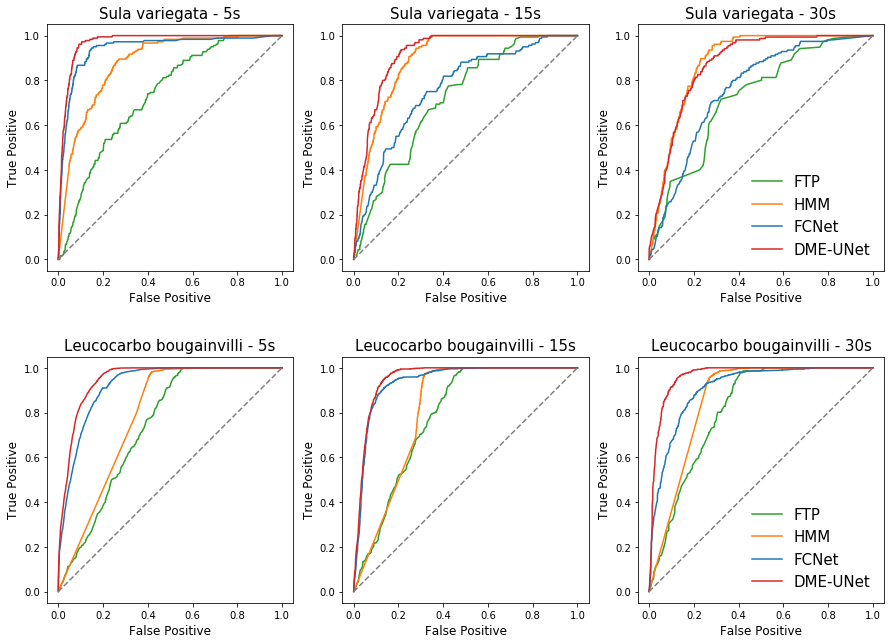
\includegraphics[scale=0.5]{figure1.png}
  \caption{\textbf{Comparison of algorithms} - ROC curves obtained from the prediction of 4 algorithms, First-Time Passage (FTP), 3-states Hidden Markov Models (HMM), Fully-Connected Network (FCN) and U-Network with a Distance Matrix Encoder (DME-UNet) on 4 distinct test datasets derived from two seabirds species breeding in Pescadores Island from 2008 to 2013}
  \label{figure1}
\end{figure}

\begin{figure}[h]
  \centering
  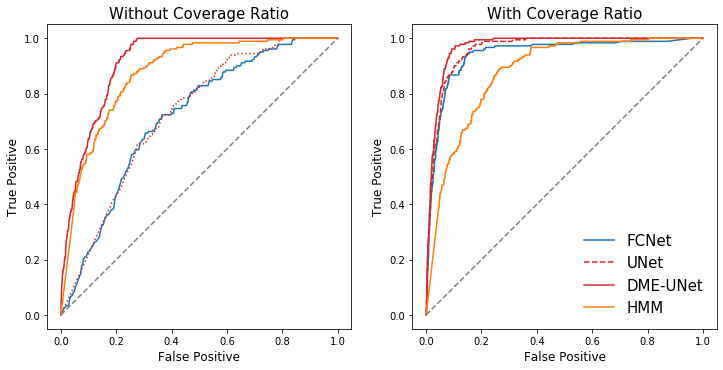
\includegraphics[scale=0.5]{figure2.png}
  \caption{\textbf{Comparison of data inputs} - ROC curves obtained from the prediction of 3 deep networks, Fully-Connected Network (FCN) and U-Network with/without a Distance Matrix Encoder (resp. UNet / DME-UNet) on the test dataset derived from Peruvian boobies sampled at 5s breeding in Pescadores Island from 2008 to 2013}
  \label{figure2}
\end{figure}

\begin{figure}[h]
  \hspace*{-2cm}
  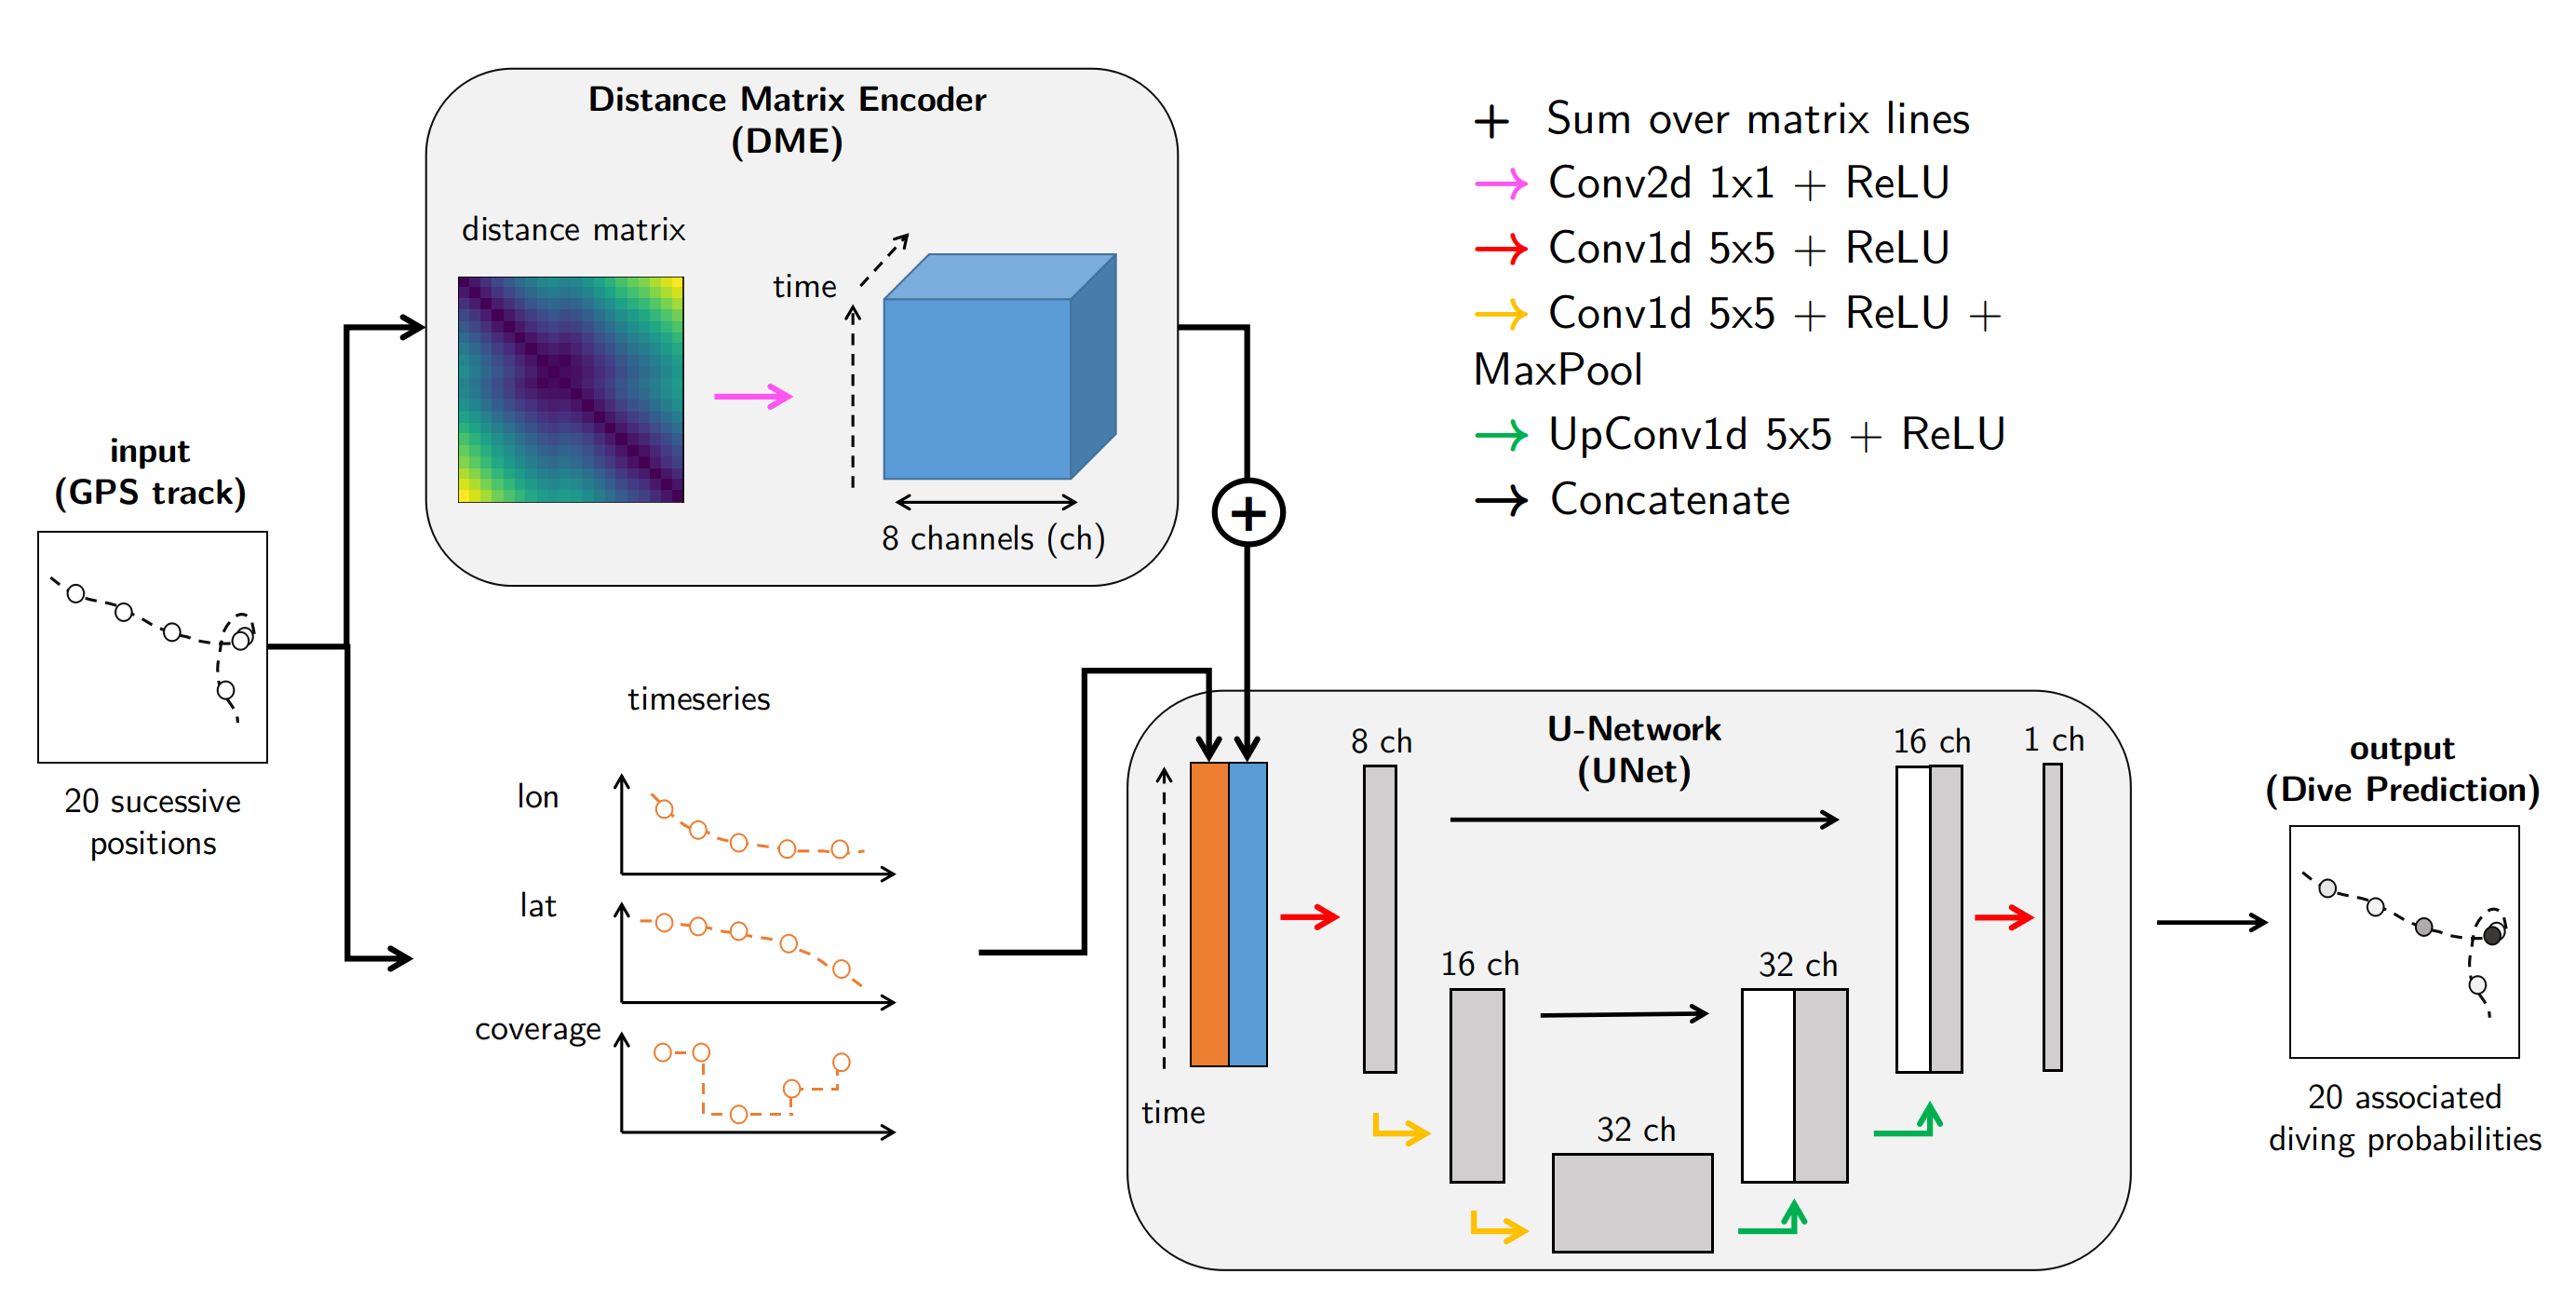
\includegraphics[scale=0.45]{figure3.png}
  \caption{\textbf{DME-UNet Architecture} - This network is composed of two blocks entitled Distance Matrix Encoder (DME) and U-Network (UNet). It takes as input a GPS of 20 successive positions and outputs a diving probability to each of these positions}
  \label{figure3}
\end{figure}

\begin{figure}[h]
  \centering
  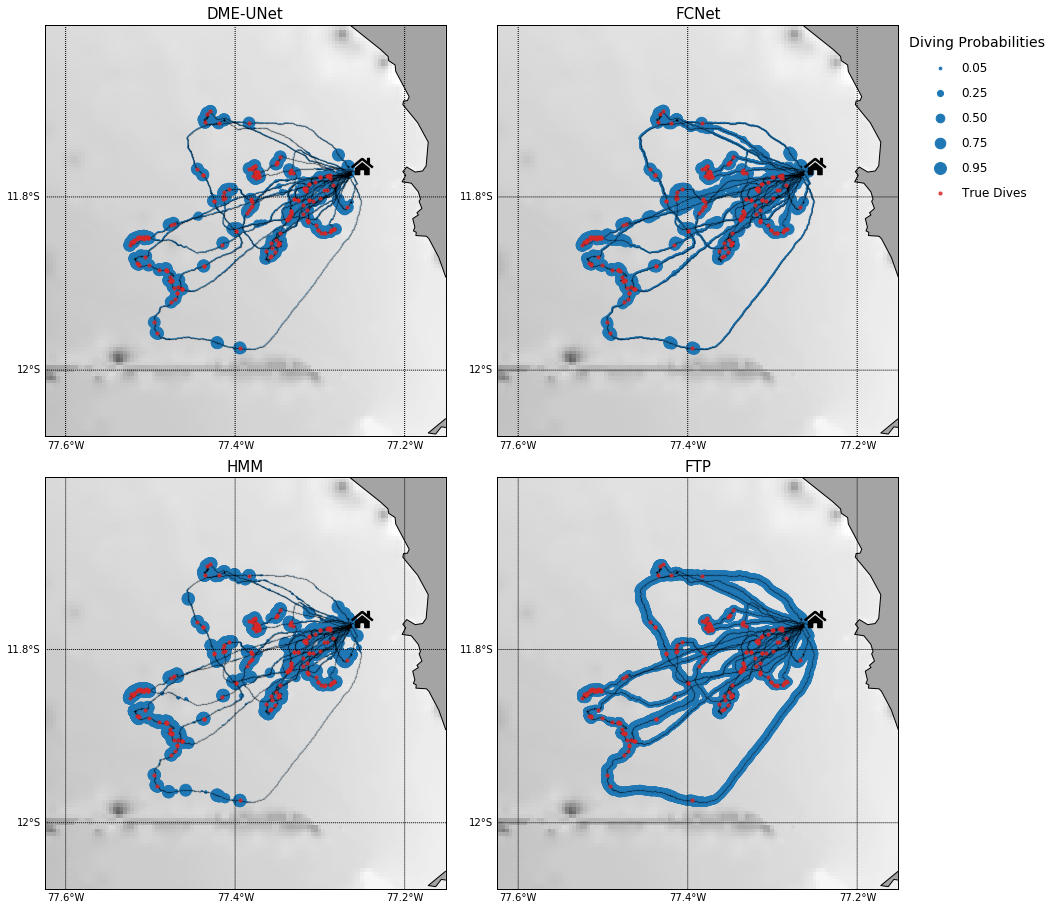
\includegraphics[scale=0.5]{figure4a.png}
  \caption{\textbf{Maps of Peruvian boobies predicted dives} - Maps of the trajectories. Red points represent true dive derived from TDR data. Blue points represents diving probabilities of each location with radius increasing for higher probabilities. These probabilities are the results of four methods on the same Dataset (SV 5s), with our proposed network DME-UNet (top left), the fully connected network used by \cite{browning_predicting_2018}  FCNet (top right), the 3 states Hidden Markov Models HMM (bottom left), and the First Time Passage apporach FTP (bottom right)}
  \label{figure4a}
\end{figure}

\begin{figure}[h]
  \centering
  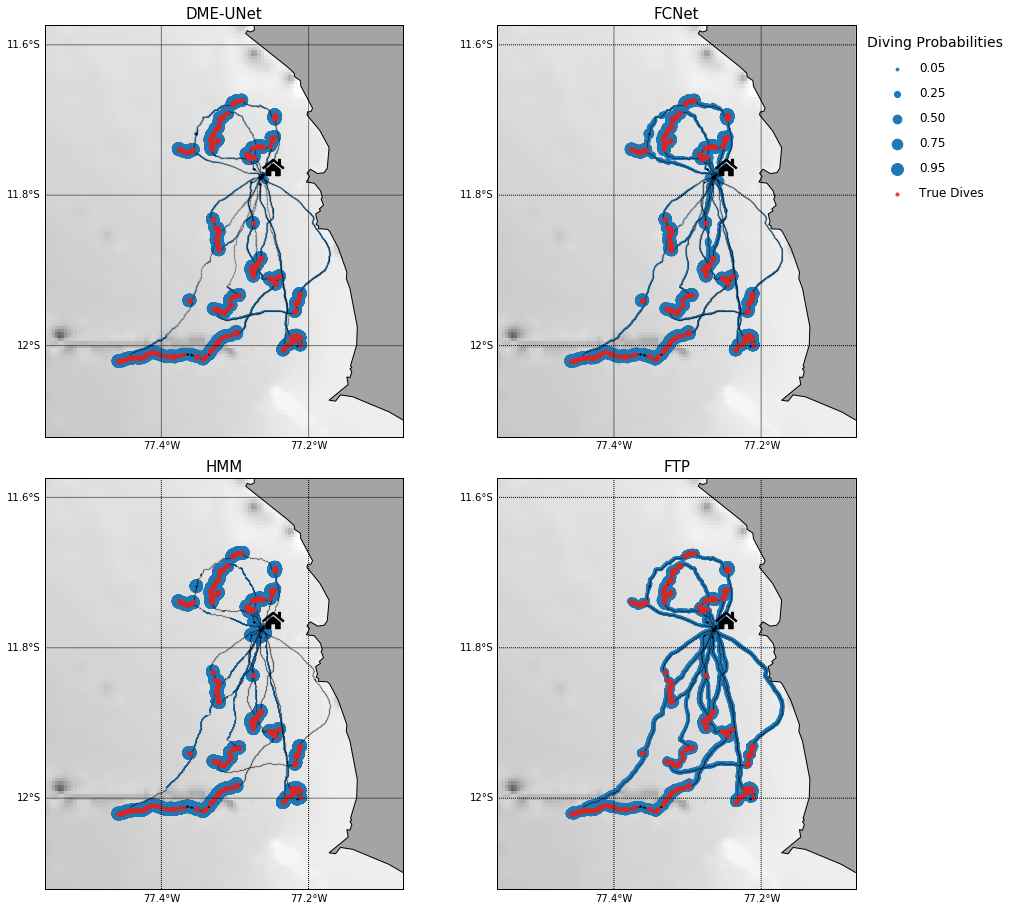
\includegraphics[scale=0.5]{figure4b.png}
  \caption{\textbf{Maps of Guanay cormorants predicted dives} - Maps of the testing trajectories. Red points represent true dive derived from TDR data. Blue points represents diving probabilities of each location with radius increasing for higher probabilities. These probabilities are the results of four methods on the same Dataset (LB 5s), with our proposed network DME-UNet (top left), the fully connected network used by \cite{browning_predicting_2018}  FCNet (top right), the 3 states Hidden Markov Models HMM (bottom left), and the First Time Passage apporach FTP (bottom right)}
  \label{figure4b}
\end{figure}

\begin{figure}[h]
  \centering
  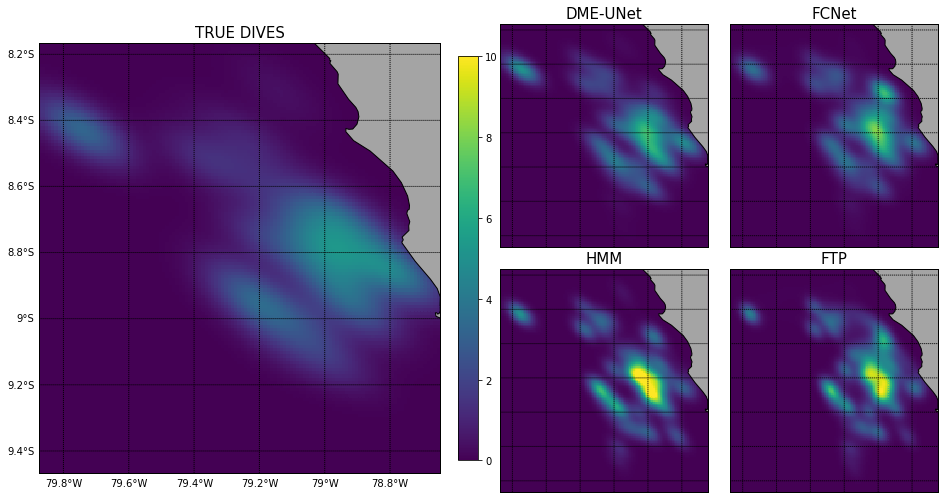
\includegraphics[scale=0.5]{figure5.png}
  \caption{\textbf{Maps of dive distributions of Peruvian Boobies from Guanape Island} - These density maps were obtained through Kernel Density Estimation. The left map has been computed from true dives derived from TDR data. The four other maps are estimations of this map, using  all points of the trajectories with weights associated to diving probabilities estimated by the four studied approaches,  with our proposed network DME-UNet (top left), the fully connected network used by \cite{browning_predicting_2018}  FCNet (top right), the 3 states Hidden Markov Models HMM (bottom left), and the First Time Passage apporach FTP (bottom right). Hellinger distance of the 4 estimations to the ground truth defined as the TRUE DIVES map are in Table \ref{table3}}
  \label{figure5}
\end{figure}

\begin{table}[h]
 \caption{\textbf{Datasets Overview} - General statistics on the three datasets used in this study. (m $\pm$ s) is for respectively mean and standard deviation}
  \centering
  \begin{tabular}{lllllll}
    \toprule
    Species  &  Colony Location & Nb of trips  & Trip Duration & Dives  & Dives Duration & Gaps \\
      &    &     & (min) & (\%) & (s) & (\%) \\
    \midrule
    \textit{Sula variegata}         & Guanape Island    & 25   & 178 $\pm$ 88  & 0.5 \%  & 3.6 $\pm$ 2.6 & 8.9 \% \\
    \textit{Sula variegata}         & Pescadores Island & 133 & 65 $\pm$ 43  & 0.8 \%  & 2.2 $\pm$ 0.9  & 13.4 \% \\
    \textit{Leucocarbo bougainvilli}& Pescadores Island & 76   & 123 $\pm$ 45  & 22.9 \%  & 17.6 $\pm$ 12.6 & 40.9 \% \\
    \bottomrule
  \end{tabular}
  \label{table1}
\end{table}

\begin{table}[h]
 \caption{\textbf{Overview of all Trained Deep Networks} - All trained deep networks on the trajectories of Pescadores are given in this table, plus other methods used for comparison. AUC means the Area Under the ROC curve, BCE is for binary cross entropy computed on the testing trajectories. Train and Validation Loss correspond to the loss estimation after model training on respectively training and validation trajectories}
  \centering
  \begin{tabular}{llllllll}
    \toprule
    Dataset  &  Resolution &  Model & Variables & AUC & BCE & Train Loss & Validation Loss \\
    \midrule
    SV       & 5s  & FTP    & lon, lat               & 0.73 & 0.65 & - & -     \\
(Pescadores) &     & HMM    & step length, direction & 0.87 & 2.98 & - & -     \\
            &     & HMM    & step length, direction, cov & 0.88 & 2.83 & - & - \\
             &     & FCNet  & lon, lat               & 0.71 & 0.52 & 1.05 & 1.12 \\
             &     & FCNet  & lon, lat, cov          & 0.94 & 0.22 & 0.42 & 0.74  \\
             &     & UNet   & lon, lat               & 0.72 & 0.48 & 0.97 & 1.12  \\
             &     & UNet   & lon, lat, cov          & 0.96 & 0.21 & 0.47 & 0.61  \\
             &     & DME-UNet   & lon, lat   & 0.92 & 0.27 & 0.57 & 0.66  \\
             &     & \textbf{DME-UNet}   & \textbf{lon, lat, cov}  & \textbf{0.97} & \textbf{0.16} & \textbf{0.36} & \textbf{0.56}  \\
             & 15s & FTP    & lon, lat               & 0.72 & 0.75 & - & -      \\
             &     & HMM    & step length, direction, cov & 0.89 & 3.36 & - & -       \\
             &     & FCNet  & lon, lat, cov          & 0.76 & 0.94 & 1.65 & 1.80 \\
             &     & \textbf{DME-UNet}   & \textbf{lon, lat, cov}  & \textbf{0.92} & \textbf{0.45} & \textbf{0.86} & \textbf{1.07}  \\
             & 30s & FTP    & lon, lat               & 0.72 & 0.89 & - & -      \\
             &     & \textbf{HMM}    & \textbf{step length, direction, cov} & \textbf{0.88} & \textbf{1.91} & \textbf{-} & \textbf{-}       \\
             &     & FCNet  & lon, lat, cov          & 0.76 & 1.30 & 2.13 & 2.40 \\
             &     & DME-UNet   & lon, lat, cov  & 0.87 & 0.82 & 1.32 & 1.52 \\
    \midrule
    LB       & 5s  & FTP    & lon, lat               & 0.74 & 0.61 & - & -        \\
(Pescadores) &     & HMM    & step length, direction, cov & 0.78 & 7.10 & - & -      \\
             &     & FCNet  & lon, lat, cov          & 0.92 & 0.44 & 0.44 & 0.47  \\
             &     & \textbf{DME-UNet}   & \textbf{lon, lat, cov}  & \textbf{0.95} & \textbf{0.36} & \textbf{0.38} & \textbf{0.39}  \\
             & 15s & FTP    & lon, lat               & 0.78 & 0.58 & - & -      \\
             &     & HMM    & step length, direction, cov & 0.81 & 4.76 & - & -  \\
             &     & FCNet  & lon, lat, cov          & 0.94 & 0.41 & 0.53 & 0.51  \\
             &     & \textbf{DME-UNet}   & \textbf{lon, lat, cov}  & \textbf{0.95} & \textbf{0.35} & \textbf{0.40} & \textbf{0.43}  \\
             & 30s & FTP    & lon, lat               & 0.82 & 0.56 & - & -      \\
             &     & HMM    & step length, direction, cov & 0.86 & 4.26 & - & - \\
             &     & FCNet  & lon, lat, cov          & 0.91 & 0.65 & 0.84 & 0.79  \\
             &     & \textbf{DME-UNet}   & \textbf{lon, lat, cov}  & \textbf{0.96} & \textbf{0.57} & \textbf{0.63} & \textbf{0.62}  \\
    \bottomrule
  \end{tabular}
  \label{table2}
\end{table}


\begin{table}[h]
 \caption{\textbf{Guanape projection} - The deep network fitted on the 5s sampled SV dataset in Pescadores have been used for dive prediction in Guanape. AUC is for area under the roc curve. BCE is the binary cross entropy. Hellinger Distance corresponds to the distance of the diving distribution maps estimated with kernel density estimations and plotted in Figure \ref{figure5} to the correct diving distribution}
  \centering
  \begin{tabular}{llllllll}
    \toprule
    Dataset  &  Resolution &  Model & Variables & AUC & BCE & Hellinger Distance \\
    \midrule
    SV      & 5s  & FTP    & lon, lat               & 0.75 & 0.47 & 32.2          \\
  (Guanape) &     & HMM    & step length, direction, cov & 0.88 & 3.70 & 29.6     \\
            &     & FCNet  & lon, lat, cov  & 0.97 & 0.10 & 25.0                  \\
            &     & DME-UNet   & lon, lat, cov  & 0.96 & 0.07 & 15.1              \\
    \bottomrule
  \end{tabular}
  \label{table3}
\end{table}


\end{document}
